\documentclass[12pt,a4paper]{standalone}
\usepackage{amssymb}
\usepackage{amsmath}
\usepackage{bm}
\usepackage{tikz}
\usetikzlibrary{arrows.meta}
\usetikzlibrary{arrows}
\usepackage{pstricks}
\usetikzlibrary{patterns}
\usetikzlibrary{fadings}
\usetikzlibrary{shapes.geometric}



\begin{document}
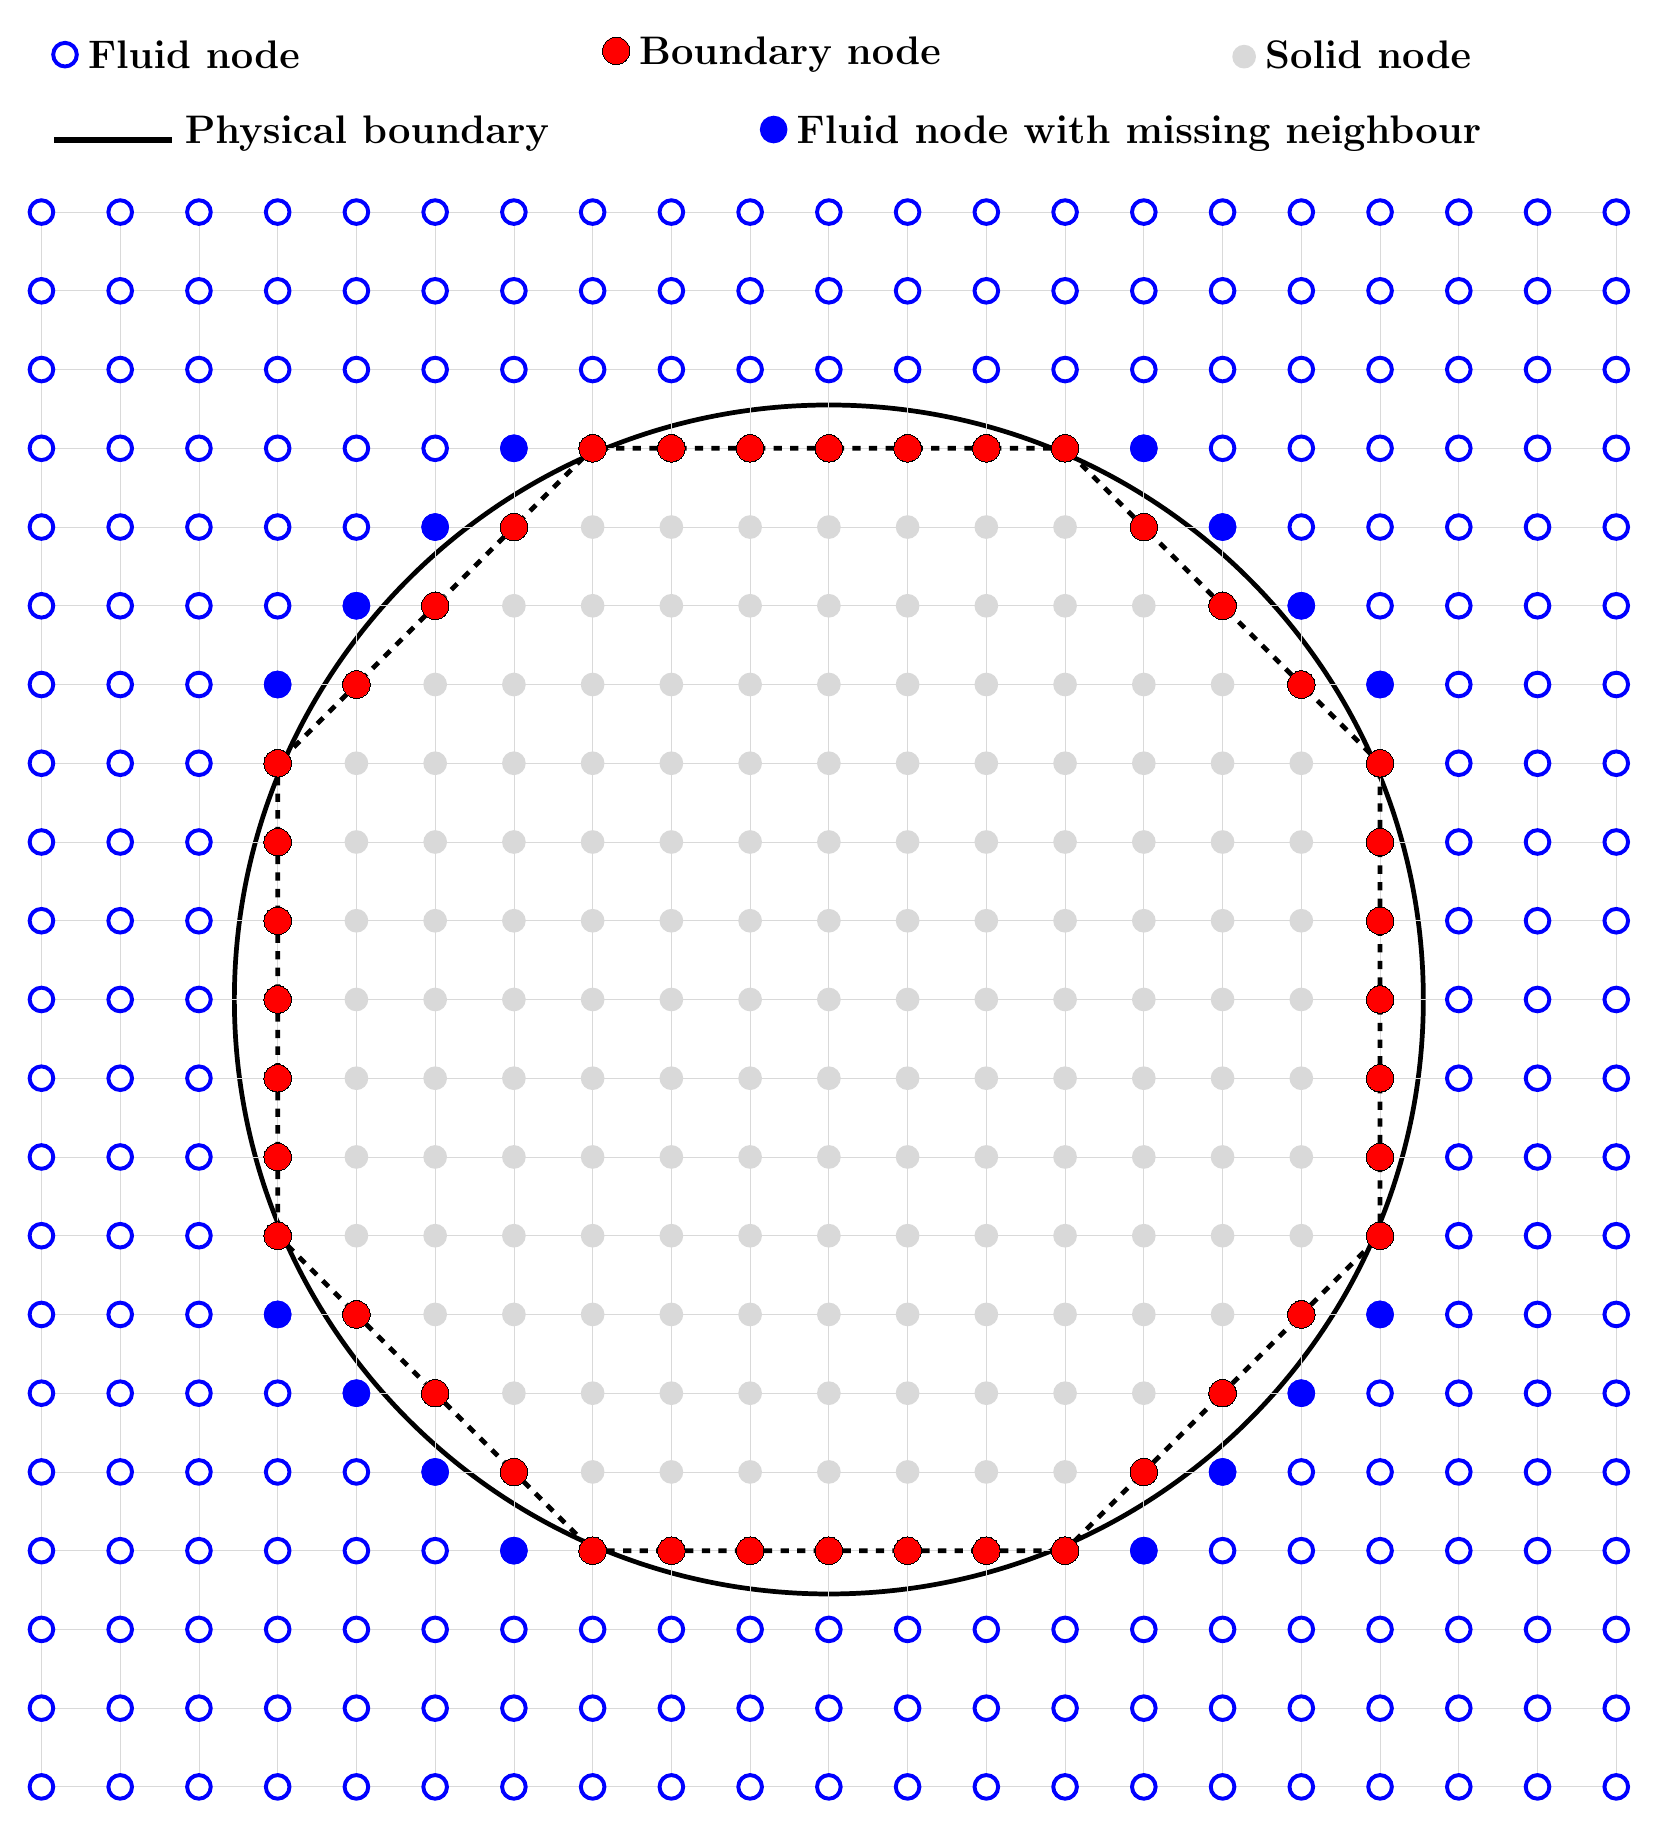
\begin{tikzpicture}[line width=0.6mm]

	%\draw[thick,line width=1mm] (17.5,10) arc[start angle=0, end angle=360, radius=7.53];
	\draw[black,fill=white] (10,10)node[]{} circle(7.55cm);

	\tikzset{myblue/.style={draw=blue, fill=white, line width=0.5mm, circle, minimum size=0.3cm, inner sep=0pt}}

	% Horizontal and vertical grid lines
	\foreach \y in {0,...,20} {
			\draw[gray!30, line width=0.1mm] (0,\y) -- (20,\y);
		}
	\foreach \x in {0,...,20} {
			\draw[gray!30, line width=0.1mm] (\x,0) -- (\x,20);
		}

	% Column 0-2 (full columns)
	\foreach \x in {0,1,2} {
			\foreach \y in {0,...,20} {
					\node[myblue] at (\x,\y) {};
				}
		}

	% Column 3
	\foreach \y in {0,...,6} { \node[myblue] at (3,\y) {}; }
	\foreach \y in {14,...,20} { \node[myblue] at (3,\y) {}; }

	% Column 4
	\foreach \y in {0,...,5} { \node[myblue] at (4,\y) {}; }
	\foreach \y in {15,...,20} { \node[myblue] at (4,\y) {}; }

	% Column 5
	\foreach \y in {0,...,4} { \node[myblue] at (5,\y) {}; }
	\foreach \y in {16,...,20} { \node[myblue] at (5,\y) {}; }

	% Column 6
	\foreach \y in {0,...,3} { \node[myblue] at (6,\y) {}; }
	\foreach \y in {17,...,20} { \node[myblue] at (6,\y) {}; }

	% Column 7
	\foreach \y in {0,...,2} { \node[myblue] at (7,\y) {}; }
	\foreach \y in {18,...,20} { \node[myblue] at (7,\y) {}; }

	% Column 8
	\foreach \y in {0,...,2} { \node[myblue] at (8,\y) {}; }
	\foreach \y in {18,...,20} { \node[myblue] at (8,\y) {}; }

	% Column 9
	\foreach \y in {0,...,2} { \node[myblue] at (9,\y) {}; }
	\foreach \y in {18,...,20} { \node[myblue] at (9,\y) {}; }

	% Column 10
	\foreach \y in {0,...,2} { \node[myblue] at (10,\y) {}; }
	\foreach \y in {18,...,20} { \node[myblue] at (10,\y) {}; }

	% Column 11
	\foreach \y in {0,...,2} { \node[myblue] at (11,\y) {}; }
	\foreach \y in {18,...,20} { \node[myblue] at (11,\y) {}; }

	% Column 12
	\foreach \y in {0,...,2} { \node[myblue] at (12,\y) {}; }
	\foreach \y in {18,...,20} { \node[myblue] at (12,\y) {}; }

	% Column 13
	\foreach \y in {0,...,2} { \node[myblue] at (13,\y) {}; }
	\foreach \y in {18,...,20} { \node[myblue] at (13,\y) {}; }

	% Column 14
	\foreach \y in {0,...,3} { \node[myblue] at (14,\y) {}; }
	\foreach \y in {17,...,20} { \node[myblue] at (14,\y) {}; }

	% Column 15
	\foreach \y in {0,...,4} { \node[myblue] at (15,\y) {}; }
	\foreach \y in {16,...,20} { \node[myblue] at (15,\y) {}; }

	% Column 16
	\foreach \y in {0,...,5} { \node[myblue] at (16,\y) {}; }
	\foreach \y in {15,...,20} { \node[myblue] at (16,\y) {}; }

	% Column 17
	\foreach \y in {0,...,6} { \node[myblue] at (17,\y) {}; }
	\foreach \y in {14,...,20} { \node[myblue] at (17,\y) {}; }

	% Column 18-20 (full columns)
	\foreach \x in {18,19,20} {
			\foreach \y in {0,...,20} {
					\node[myblue] at (\x,\y) {};
				}
		}

	%Boundary nodes

	\tikzset{mydot/.style={draw=black, fill=red, line width=0mm, circle, minimum size=0.35cm, inner sep=0pt}}

	% Draw the dots
	\node[mydot] (p1) at (3,8) {};
	\node[mydot] (p2) at (3,9) {};
	\node[mydot] (p3) at (3,10) {};
	\node[mydot] (p4) at (3,11) {};
	\node[mydot] (p5) at (3,12) {};
	\node[mydot] (p6) at (3,13) {};

	\node[mydot] (p7) at (3,7) {};
	\node[mydot] (p8) at (4,6) {};
	\node[mydot] (p9) at (5,5) {};
	\node[mydot] (p10) at (6,4) {};

	\node[mydot] (p11) at (7,3) {};
	\node[mydot] (p12) at (8,3) {};
	\node[mydot] (p13) at (9,3) {};
	\node[mydot] (p14) at (10,3) {};
	\node[mydot] (p15) at (11,3) {};
	\node[mydot] (p16) at (12,3) {};
	\node[mydot] (p17) at (13,3) {};

	\node[mydot] (p18) at (14,4) {};
	\node[mydot] (p19) at (15,5) {};
	\node[mydot] (p20) at (16,6) {};
	\node[mydot] (p21) at (17,7) {};
	\node[mydot] (p22) at (17,8) {};
	\node[mydot] (p23) at (17,9) {};
	\node[mydot] (p24) at (17,10) {};
	\node[mydot] (p25) at (17,11) {};
	\node[mydot] (p26) at (17,12) {};
	\node[mydot] (p27) at (17,13) {};

	\node[mydot] (p28) at (16,14) {};
	\node[mydot] (p29) at (15,15) {};
	\node[mydot] (p30) at (14,16) {};
	\node[mydot] (p31) at (13,17) {};
	\node[mydot] (p32) at (12,17) {};
	\node[mydot] (p33) at (11,17) {};
	\node[mydot] (p34) at (10,17) {};
	\node[mydot] (p35) at (9,17) {};
	\node[mydot] (p36) at (8,17) {};
	\node[mydot] (p37) at (7,17) {};
	\node[mydot] (p38) at (6,16) {};
	\node[mydot] (p39) at (5,15) {};
	\node[mydot] (p40) at (4,14) {};

	% Connect with dashed line
	\draw[dashed] (p7) -- (p8) -- (p9) -- (p10) -- (p11) -- (p12) -- (p13) -- (p14) -- (p15) -- (p16) -- (p17) --
	(p18) -- (p19) -- (p20) -- (p21) -- (p22) -- (p23) -- (p24) -- (p25) -- (p26) -- (p27) --
	(p28) -- (p29) -- (p30) -- (p31) -- (p32) -- (p33) -- (p34) -- (p35) -- (p36) -- (p37) --
	(p38) -- (p39) -- (p40) -- (p6) -- (p5) -- (p4) -- (p3) -- (p2) -- (p1) -- (p7) -- cycle;

	%Bc fluid
	\tikzset{myblue2/.style={draw=blue, fill=blue, line width=0.5mm, circle, minimum size=0.3cm, inner sep=0pt}}
	\tikzset{mygray/.style={draw=gray!30, fill=gray!30, line width=0.5mm, circle, minimum size=0.25cm, inner sep=0pt}}

	\node[myblue2] at (3,6) {};
	\node[myblue2] at (4,5) {};
	\node[myblue2] at (5,4) {};
	\node[myblue2] at (6,3) {};

	\node[myblue2] at (14,3) {};
	\node[myblue2] at (15,4) {};
	\node[myblue2] at (16,5) {};
	\node[myblue2] at (17,6) {};

	\node[myblue2] at (3,14) {};
	\node[myblue2] at (4,15) {};
	\node[myblue2] at (5,16) {};
	\node[myblue2] at (6,17) {};

	\node[myblue2] at (17,14) {};
	\node[myblue2] at (16,15) {};
	\node[myblue2] at (15,16) {};
	\node[myblue2] at (14,17) {};

	\foreach \y in {7,...,13} { \node[mygray] at (4,\y) {}; }
	\foreach \y in {6,...,14} { \node[mygray] at (5,\y) {}; }
	\foreach \y in {5,...,15} { \node[mygray] at (6,\y) {}; }
	\foreach \y in {4,...,16} { \node[mygray] at (7,\y) {}; }
	\foreach \y in {4,...,16} { \node[mygray] at (8,\y) {}; }
	\foreach \y in {4,...,16} { \node[mygray] at (9,\y) {}; }
	\foreach \y in {4,...,16} { \node[mygray] at (10,\y) {}; }
	\foreach \y in {4,...,16} { \node[mygray] at (11,\y) {}; }
	\foreach \y in {4,...,16} { \node[mygray] at (12,\y) {}; }
	\foreach \y in {4,...,16} { \node[mygray] at (13,\y) {}; }
	\foreach \y in {5,...,15} { \node[mygray] at (14,\y) {}; }
	\foreach \y in {6,...,14} { \node[mygray] at (15,\y) {}; }
	\foreach \y in {7,...,13} { \node[mygray] at (16,\y) {}; }

	%\node[draw=gray, fill=gray, minimum size=0.3cm] at (17,6) {};

	%\node [draw, gray, fill=white,diamond, aspect=1,scale=0.8] at (6,8) {};
	%\node [draw, gray, fill=white,diamond, aspect=1,scale=0.8] at (6,10) {};
	%\node [draw, gray, fill=white,diamond, aspect=1,scale=0.8] at (6,12) {};

	\draw (0,22) node[anchor=west] { \tikz{\node[myblue] {};} {\Large\textbf{Fluid node}} };
	\draw (7,22) node[anchor=west] { \tikz{\node[mydot] {};} {\Large\textbf{Boundary node}} };
	\draw (15,22) node[anchor=west] { \tikz{\node[mygray] {};} {\Large\textbf{Solid node}} };
	\draw (9,21) node[anchor=west] { \tikz{\node[myblue2] {};} {\Large\textbf{Fluid node with missing neighbour}} };
	\draw (0,21) node[anchor=west] { \tikz{\draw[black,thick, line width=0.8mm] (0,0.8) -- (1.5,0.8);} {\Large\textbf{Physical boundary}} };

	%\draw (7,7)node[]{{\LARGE{\textbf{Solid}}}};
	%\draw (4.5,15.5)node[rotate=45]{{\LARGE{\textbf{Wall}}}};

	% \draw[dashed,thick,line width=0.2mm] (4,2) -- (7.7,7.4);

	% \draw[gray,solid,thick,line width=0.2mm] (0,0) -- (13,0);
	% \draw[gray,solid,thick,line width=0.2mm] (1,2) -- (13,2);
	% \draw[gray,solid,thick,line width=0.2mm] (1,4) -- (13,4);
	% \draw[gray,solid,thick,line width=0.2mm] (1,6) -- (13,6);
	% \draw[gray,solid,thick,line width=0.2mm] (1,8) -- (13,8);
	%
	% \draw[gray,solid,thick,line width=0.2mm] (2,-1) -- (2,9);
	% \draw[gray,solid,thick,line width=0.2mm] (4,-1) -- (4,9);
	% \draw[gray,solid,thick,line width=0.2mm] (6,-1) -- (6,9);
	% \draw[gray,solid,thick,line width=0.2mm] (8,-1) -- (8,9);
	% \draw[gray,solid,thick,line width=0.2mm] (10,-1) -- (10,9);
	% \draw[gray,solid,thick,line width=0.2mm] (12,-1) -- (12,9);

	% \draw[thick,line width=1mm] (8.2,-0.4) arc[start angle=15, end angle=85, radius=8];
	% \draw[pattern=north west lines, pattern color=white] (6,4) rectangle (8,6);
	% \draw[pattern=north east lines, pattern color=gray] (6,6) rectangle (8,8);

	% %top first row
	% \draw[black,fill=white] (2,8)node[]{} circle(0.2cm);
	% \draw[black,fill=white] (4,8)node[]{} circle(0.15cm);
	% \draw[black,fill=white] (6,8)node[]{} circle(0.15cm);
	% \draw[black,fill=white] (8,8)node[]{} circle(0.15cm);
	% \draw[black,fill=white] (10,8)node[]{} circle(0.15cm);
	% \draw[black,fill=white] (12,8)node[]{} circle(0.15cm);
	%
	% %top second row
	% \draw[black,fill=white] (2,6)node[]{} circle(0.15cm);
	% \draw[black,fill=white] (4,6)node[]{} circle(0.15cm);
	% \draw[black,fill=white] (6,6)node[]{} circle(0.15cm);
	% \draw[black,fill=white] (8,6)node[]{} circle(0.15cm);
	% \draw[black,fill=white] (10,6)node[]{} circle(0.15cm);
	% \draw[black,fill=white] (12,6)node[]{} circle(0.15cm);
	%
	% %top third row
	% \draw[black,fill=black] (2,4)node[]{} circle(0.15cm);
	% \draw[black,fill=black] (4,4)node[]{} circle(0.15cm);
	% \draw[black,fill=white] (6,4)node[]{} circle(0.15cm);
	% \draw[black,fill=white] (8,4)node[]{} circle(0.15cm);
	% \draw[black,fill=white] (10,4)node[]{} circle(0.15cm);
	% \draw[black,fill=white] (12,4)node[]{} circle(0.15cm);
	%
	% %top fourth row
	% \draw[black,fill=black] (4,2)node[]{} circle(0.15cm);
	% \draw[black,fill=black] (6,2)node[]{} circle(0.15cm);
	% \draw[black,fill=white] (8,2)node[]{} circle(0.15cm);
	% \draw[black,fill=white] (10,2)node[]{} circle(0.15cm);
	% \draw[black,fill=white] (12,2)node[]{} circle(0.15cm);
	%
	% %top fifth row
	% \draw[black,fill=black] (6,0)node[]{} circle(0.15cm);
	% \draw[black,fill=black] (8,0)node[]{} circle(0.15cm);
	% \draw[black,fill=white] (10,0)node[]{} circle(0.15cm);
	% \draw[black,fill=white] (12,0)node[]{} circle(0.15cm);

	% \node [draw, fill=gray,diamond, aspect=1,scale=0.7] at (5.22,3.78) {};
	% \node [draw, fill=gray,diamond, aspect=1,scale=0.7] at (6.4,5.5) {};
	% \node [draw, fill=gray,diamond, aspect=1,scale=0.7] at (7.7,7.4) {};
	%
	% \draw (7,5.2)node[]{\large{$\bm{P_{f1}}$}};
	% \draw (8.4,7.4)node[]{\large{$\bm{P_{f2}}$}};
	%
	%
	% \draw (5.7,5)node[]{\Large{$\delta_r$}};
	% \draw (7,7)node[]{\Large{$\delta_r$}};
	% \draw (4.3,3.2)node[]{\Large{$\Delta$}};
	%
	%
	% \draw (4.3,1.6)node[]{\Large{$\bm{b}$}};
	% \draw (2.7,1.5)node[]{{\textbf{boundary}}};
	% \draw (2.9,1)node[]{\textbf{node}};

	% \draw (5.8,4.3)node[]{\large{$\bm{f}$}};
	% \draw (6.8,3.6)node[]{\textbf{fluid}};
	% \draw (6.8,3.1)node[]{\textbf{node}};

	% \draw (7.6,6.3)node[]{\large{$\bm{ff}$}};

	% \draw (5.2,4.3)node[]{\Large{$\bm{w}$}};
	% \draw (5.4,3)node[]{{\textbf{wall}}};
	% \draw (5.64,2.5)node[]{{\textbf{point}}};
	%
	% \draw (1.9,4.7)node[]{{\textbf{physical}}};
	% \draw (2.4,4.25)node[]{{\textbf{boundary}}};

\end{tikzpicture}

\end{document}

